\documentclass[11pt,a4paper]{article}
\usepackage[margin=2.2cm]{geometry}
\usepackage{graphicx,booktabs,url,amsmath}
\usepackage[hidelinks]{hyperref}
\usepackage{placeins}
\usepackage{float}
\graphicspath{{../../../fullsim_analysis/results/bench/2026-10-27/}}
\newcommand{\results}{../../../fullsim_analysis/results/bench/2026-10-27}
\title{Threshold and hold delay of the Citiroc front end:\\ menu 2 of 27 October 2026}
\author{J.\,J.~Gómez-Cadenas}
\date{28 October 2026}
\begin{document}
\maketitle

\begin{center}
\small
\begin{tabular}{lp{0.72\textwidth}}
\toprule
session & 27 October 2026, menu 2 of the Citiroc~1A calibration programme \\
board & 1 (A5202, CAEN adapter board, FPGA firmware 0xa7070800) \\
SiPMs & 43~V, 5~V of overvoltage \\
measurements & one threshold scan (staircase), six hold-delay scans at 25 and 50~ns \\
this report & threshold of the discriminator; response of the peak detector to one
  avalanche; minimum hold delay at 25 and 50~ns; single-photoelectron gain at 5~V \\
\bottomrule
\end{tabular}
\end{center}

\section{Data}

\begin{itemize}
\item Settings common to all scans: HV\_Vbias 47.2~V (43~V at the SiPM); TD\_CoarseThreshold
  185; preamplifier gains 55; peak-stretch mode; low gain at 87.5~ns.
\item Staircase (scan 100): trigger rate of each of the 64 channels against the threshold of
  its discriminator, 150 to 300 DAC units in steps of 1, 0.5~s per point, 25~ns.
\item Hold-delay scans (Table~\ref{tab:scans}): trigger limited to one channel (the shooting
  channel); the high-gain spectrum of every channel stored at each delay; 10\,000 events per
  delay.
\item The DAQ applies a new delay with a lag of up to five points: the first points of each
  scan but the first keep the values of the last delay of the previous scan. They are flagged
  (Section~\ref{sec:method}) and left out.
\end{itemize}

\begin{table}[H]
\centering
\small
\begin{tabular}{llllc}
\toprule
Scan & Shooting channel & HG shaping & HoldDelay & stale points \\
\midrule
101 & 0 & 25 ns & 0--248 ns in steps of 8 & 0 \\
102 & 0 & 50 ns & 0--496 ns in steps of 16 & 5 \\
103 & 0 & 50 ns & 0--496 ns in steps of 16 & 5 \\
104 & 20 & 25 ns & 0--248 ns in steps of 8 & 4 \\
105 & 40 & 25 ns & 0--248 ns in steps of 8 & 2 \\
106 & 60 & 25 ns & 0--248 ns in steps of 8 & 1 \\
\bottomrule
\end{tabular}
\caption{Hold-delay scans of 27 October, board 1, and the number of points at the start of
each scan still at the delay of the previous scan.}
\label{tab:scans}
\end{table}

\section{Method}
\label{sec:method}

Staircase: for channel $i$ and threshold $\theta$ (DAC units), with $R_i(\theta)$ the trigger
rate,
\begin{align*}
R_i^\mathrm{max} &= \max_\theta R_i(\theta), &
\theta_i^\mathrm{e} &= \max\{\theta : R_i(\theta) \ge R_i^\mathrm{max}/2\}, &
\Delta\theta &= \text{distance between consecutive steps of } R_i(\theta),
\end{align*}
\begin{itemize}
\item $R_i^\mathrm{max}$ the plateau, where the discriminator triggers on the noise of the fast
  shaper; $\theta_i^\mathrm{e}$ the edge of the plateau; $\Delta\theta$ one photoelectron in
  DAC units.
\end{itemize}

Hold-delay scan: for the shooting channel $i$ at delay $\tau$, with $S_i(v;\tau)$ its
high-gain spectrum (bins of 16 counts) and $p_i$ its pedestal below breakdown at the same
shaping,
\begin{align*}
q_1(\tau) &= \arg\max_{p_i + 48 \le v \le p_i + 400} S_i(v;\tau) \ \text{(parabolic refinement)}, &
G &= \operatorname{median}_{\text{last 8 points}} q_1(\tau) - p_i, \\
\tau_\mathrm{min} &= \min\{\tau : q_1(\tau) - p_i \ge 0.95\,G\}, &
\bar{v}_i(\tau) &= \text{mean of } S_i(v;\tau),
\end{align*}
\begin{itemize}
\item $q_1(\tau)$ the position of the 1-pe peak: the response of the peak detector to one
  avalanche, read on the peak and not on the mean $\bar{v}_i$, which also collects the dark
  pulses and the crosstalk inside the window;
\item $G$ the plateau of the 1-pe peak above the pedestal: the single-photoelectron gain;
\item $\tau_\mathrm{min}$ the knee of the response: the minimum hold delay;
\item stale points: those before the minimum over the scan of the median of $\bar{v}_j(\tau)$
  over the non-shooting channels $j$;
\item model of the front end: the shaped pulse reaches its maximum 31~ns (25~ns of shaping)
  and 58~ns (50~ns) after the crossing of the threshold.
\end{itemize}

\section{Results}

\subsection{Threshold}

\begin{figure}[H]
\centering
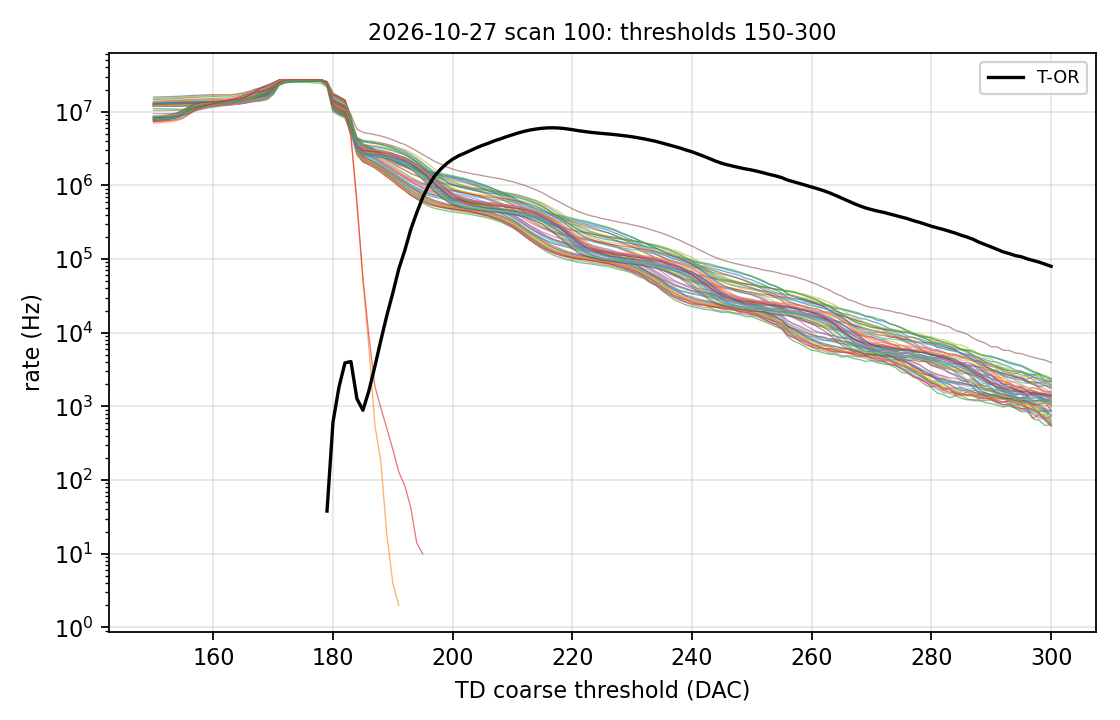
\includegraphics[width=0.8\textwidth]{staircase_100.png}
\caption{Scan 100, 25~ns, 5~V: $R_i(\theta)$ of the 64 channels of board 1 and the rate of the
OR of the 64 channels.}
\label{fig:staircase}
\end{figure}

\begin{center}
\small
\begin{tabular}{ll}
\toprule
edge $\theta^\mathrm{e}$ & 179 (median), 179--182 \\
one photoelectron $\Delta\theta$ & 20 DAC units \\
rate 30 units above the edge & $4.4\times 10^{5}$~Hz (median) \\
blind channels & 61, 63: below $10^{3}$~Hz within 10 units of the edge \\
threshold of the scans, 185 & 4--6 units above the edge, below one photoelectron \\
\bottomrule
\end{tabular}
\end{center}

\subsection{Response of the peak detector}

\begin{figure}[H]
\centering
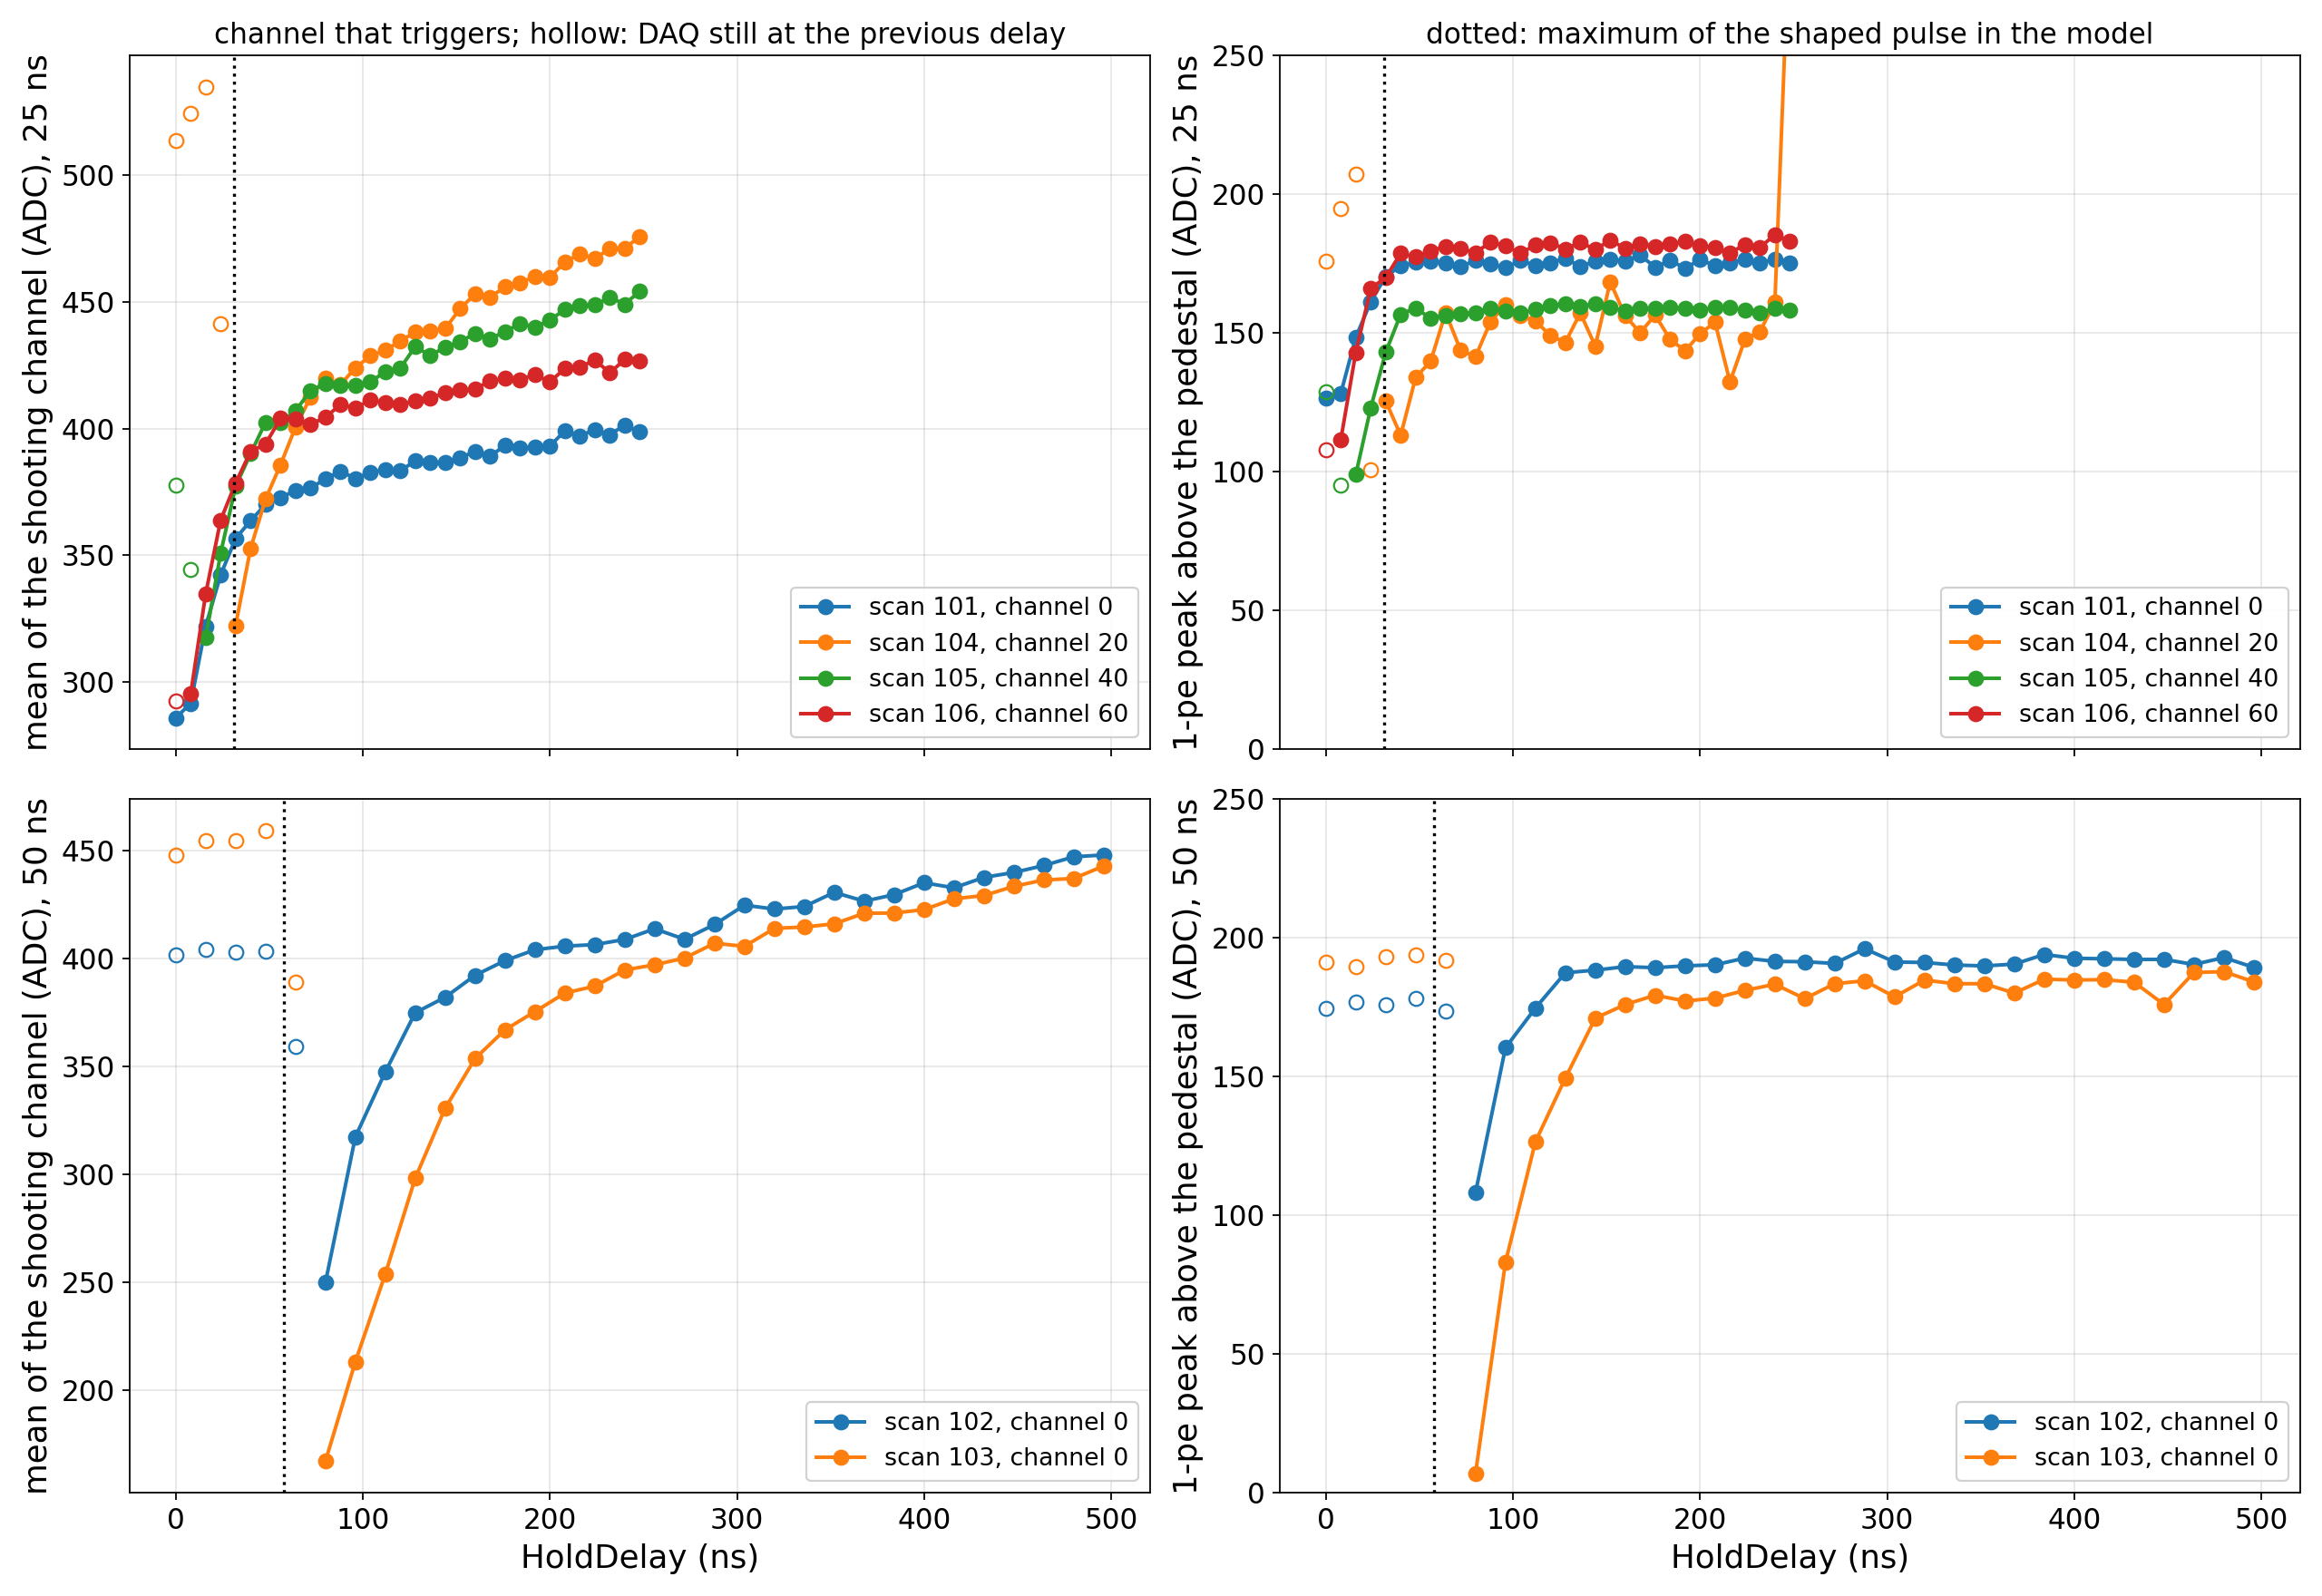
\includegraphics[width=0.95\textwidth]{hold_scan_response.png}
\caption{Hold-delay scans of board 1 at 25~ns (top) and 50~ns (bottom). Left: mean
$\bar{v}_i(\tau)$ of the shooting channel. Right: $q_1(\tau) - p_i$. Hollow: stale points.
Dotted: the maximum of the shaped pulse in the model.}
\label{fig:response}
\end{figure}

\begin{figure}[H]
\centering
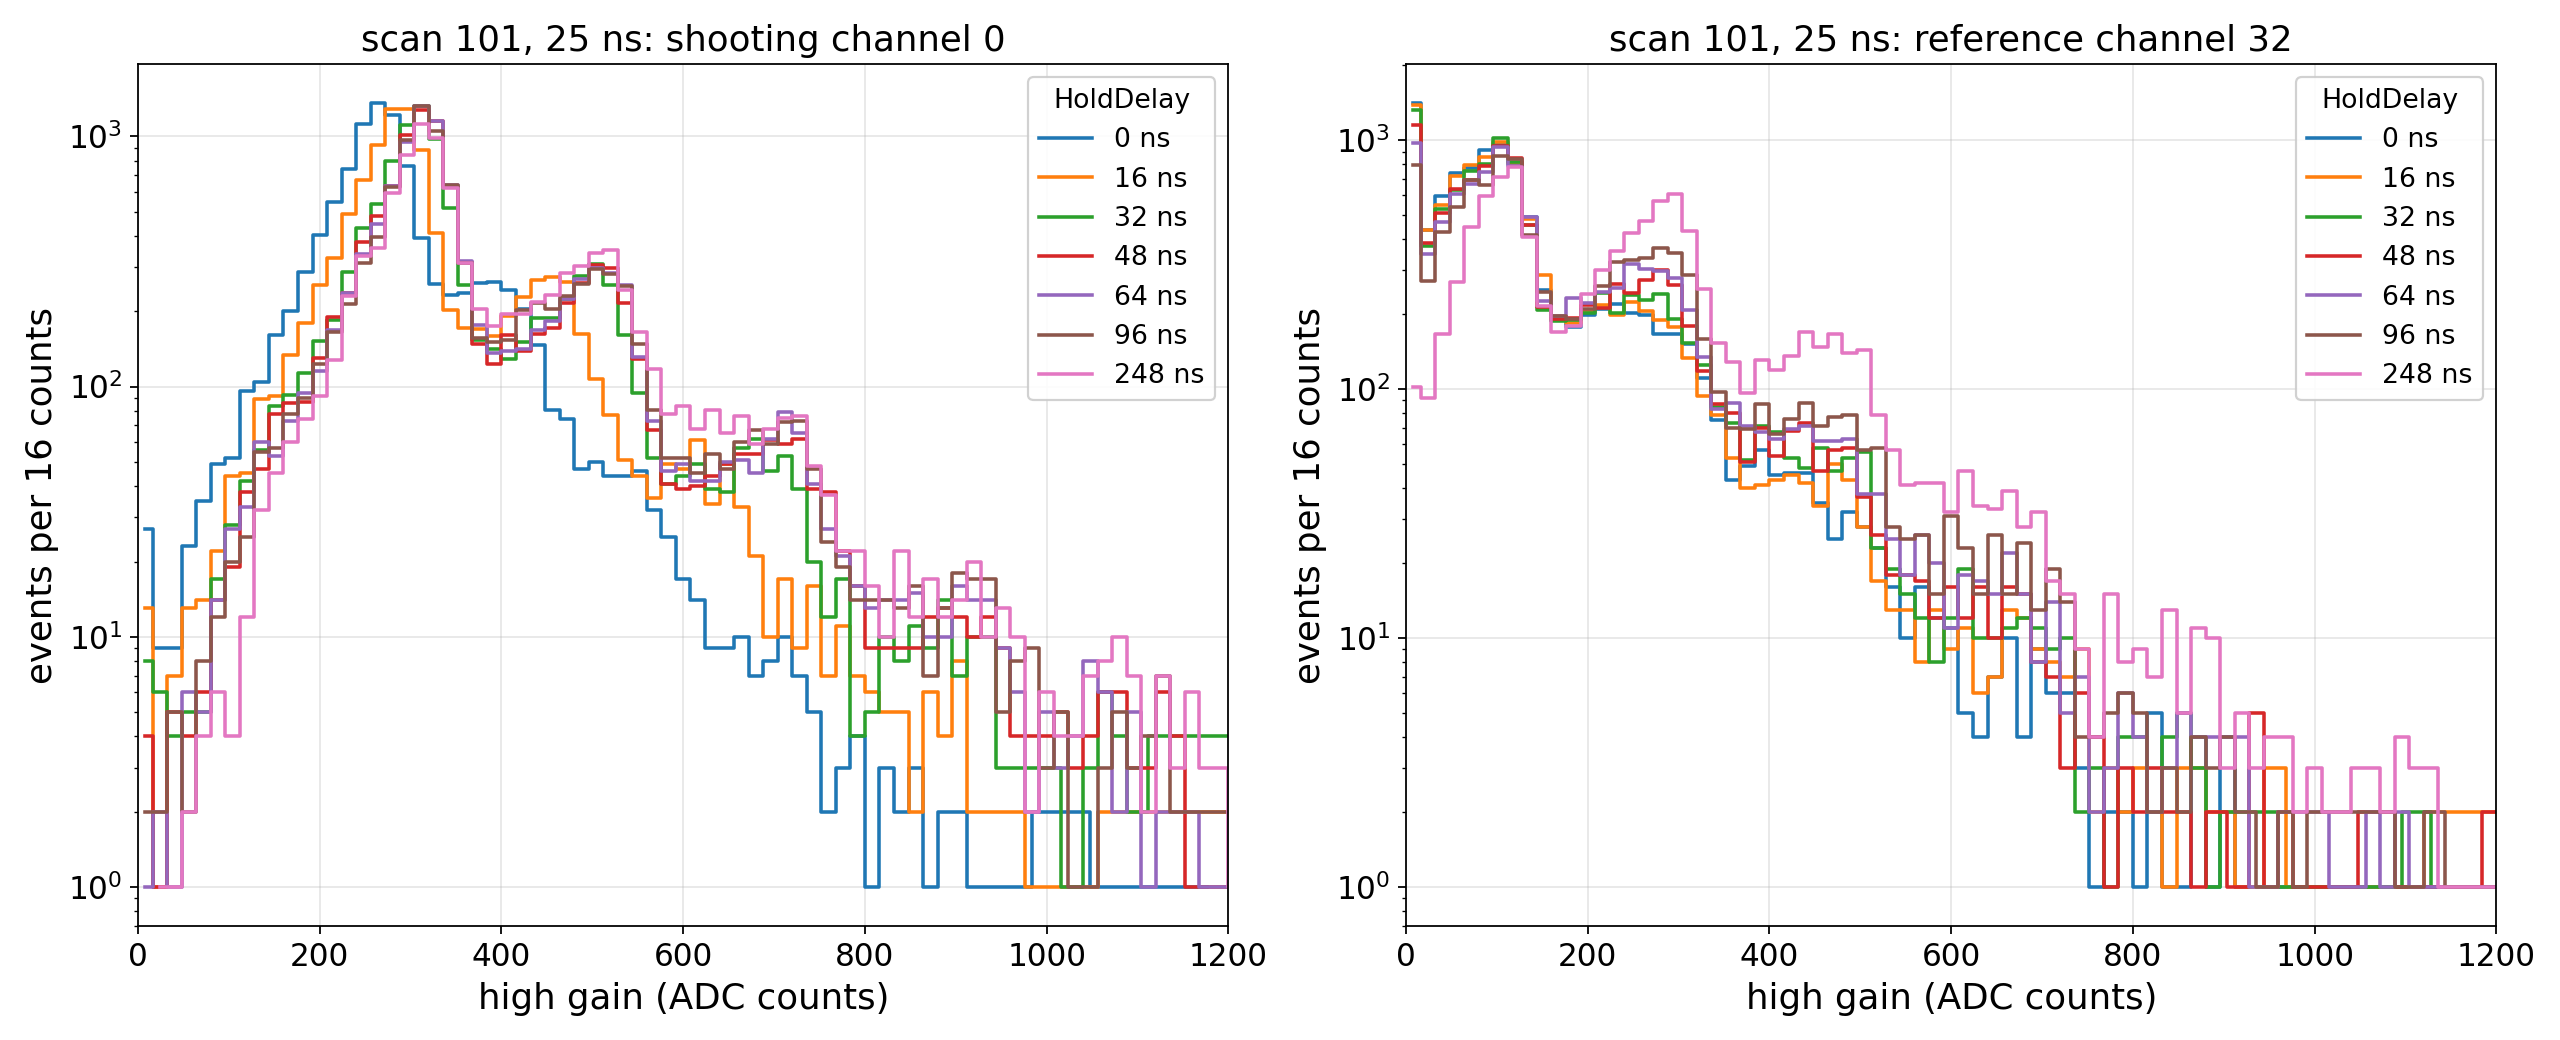
\includegraphics[width=0.95\textwidth]{hold_scan_spectra.png}
\caption{Scan 101 (25~ns): $S_i(v;\tau)$ of the shooting channel 0 (left) and of channel 32,
which does not trigger (right), at a few delays.}
\label{fig:spectra}
\end{figure}

\begin{table}[H]
\centering
\small
\input{\results/hold_scan_knees.tex}
\caption{Each scan: pedestal $p_i$, knee $\tau_\mathrm{min}$ and gain $G$ of the shooting
channel, ADC counts of the high gain.}
\label{tab:knees}
\end{table}

\begin{itemize}
\item 25~ns: $q_1$ rises from the pedestal region to its plateau at 32 to 40~ns in the four
  channels and stays flat to 248~ns (Figure~\ref{fig:response}, Table~\ref{tab:knees}); the
  model's maximum is at 31~ns.
\item 50~ns: $q_1$ reaches its plateau at 128 to 160~ns; the model's maximum is at 58~ns.
\item $\bar{v}_i$ rises with $q_1$ and keeps growing after the knee.
\item Scan 101 (Figure~\ref{fig:spectra}): 1-pe peak at 265 counts at $\tau = 0$, at 315 from
  32~ns on; 2 and 3~pe at 505 and 700, 190 counts apart.
\item Gain $G$ at 5~V: 175, 150, 159 and 182 counts per photoelectron in channels 0, 20, 40
  and 60 at 25~ns; 185 and 192 in channel 0 at 50~ns.
\end{itemize}

\section{Values}

\begin{center}
\small
\begin{tabular}{p{0.3\textwidth}p{0.55\textwidth}}
\toprule
threshold, 5~V, 25~ns & edge of the noise at 179--182 DAC units; one photoelectron = 20 units;
  185 is below one photoelectron \\
minimum hold delay & 40~ns at 25~ns of shaping; 160~ns at 50~ns \\
gain at 5~V, high gain, preamplifier gain 55 & 150--182 counts per photoelectron at 25~ns
  (four channels); 185--192 at 50~ns \\
\bottomrule
\end{tabular}
\end{center}

\end{document}
